% Options for packages loaded elsewhere
\PassOptionsToPackage{unicode}{hyperref}
\PassOptionsToPackage{hyphens}{url}
%
\documentclass[
  ignorenonframetext,
]{beamer}
\title{Week 10: Intro to Statistics}
\author{Prof.~Sara K. Yeo \textbar{} COMM 3710 \textbar{} Spring 2022}
\date{}

\usepackage{pgfpages}
\setbeamertemplate{caption}[numbered]
\setbeamertemplate{caption label separator}{: }
\setbeamercolor{caption name}{fg=normal text.fg}
\beamertemplatenavigationsymbolsempty
% Prevent slide breaks in the middle of a paragraph
\widowpenalties 1 10000
\raggedbottom
\setbeamertemplate{part page}{
  \centering
  \begin{beamercolorbox}[sep=16pt,center]{part title}
    \usebeamerfont{part title}\insertpart\par
  \end{beamercolorbox}
}
\setbeamertemplate{section page}{
  \centering
  \begin{beamercolorbox}[sep=12pt,center]{part title}
    \usebeamerfont{section title}\insertsection\par
  \end{beamercolorbox}
}
\setbeamertemplate{subsection page}{
  \centering
  \begin{beamercolorbox}[sep=8pt,center]{part title}
    \usebeamerfont{subsection title}\insertsubsection\par
  \end{beamercolorbox}
}
\AtBeginPart{
  \frame{\partpage}
}
\AtBeginSection{
  \ifbibliography
  \else
    \frame{\sectionpage}
  \fi
}
\AtBeginSubsection{
  \frame{\subsectionpage}
}
\usepackage{amsmath,amssymb}
\usepackage{lmodern}
\usepackage{iftex}
\ifPDFTeX
  \usepackage[T1]{fontenc}
  \usepackage[utf8]{inputenc}
  \usepackage{textcomp} % provide euro and other symbols
\else % if luatex or xetex
  \usepackage{unicode-math}
  \defaultfontfeatures{Scale=MatchLowercase}
  \defaultfontfeatures[\rmfamily]{Ligatures=TeX,Scale=1}
\fi
% Use upquote if available, for straight quotes in verbatim environments
\IfFileExists{upquote.sty}{\usepackage{upquote}}{}
\IfFileExists{microtype.sty}{% use microtype if available
  \usepackage[]{microtype}
  \UseMicrotypeSet[protrusion]{basicmath} % disable protrusion for tt fonts
}{}
\makeatletter
\@ifundefined{KOMAClassName}{% if non-KOMA class
  \IfFileExists{parskip.sty}{%
    \usepackage{parskip}
  }{% else
    \setlength{\parindent}{0pt}
    \setlength{\parskip}{6pt plus 2pt minus 1pt}}
}{% if KOMA class
  \KOMAoptions{parskip=half}}
\makeatother
\usepackage{xcolor}
\IfFileExists{xurl.sty}{\usepackage{xurl}}{} % add URL line breaks if available
\IfFileExists{bookmark.sty}{\usepackage{bookmark}}{\usepackage{hyperref}}
\hypersetup{
  pdftitle={Week 10: Intro to Statistics},
  pdfauthor={Prof.~Sara K. Yeo \textbar{} COMM 3710 \textbar{} Spring 2022},
  hidelinks,
  pdfcreator={LaTeX via pandoc}}
\urlstyle{same} % disable monospaced font for URLs
\newif\ifbibliography
\setlength{\emergencystretch}{3em} % prevent overfull lines
\providecommand{\tightlist}{%
  \setlength{\itemsep}{0pt}\setlength{\parskip}{0pt}}
\setcounter{secnumdepth}{-\maxdimen} % remove section numbering
\ifLuaTeX
  \usepackage{selnolig}  % disable illegal ligatures
\fi

\begin{document}
\frame{\titlepage}

\begin{frame}
\end{frame}

\hypertarget{why-statistics}{%
\section{Why statistics?}\label{why-statistics}}

\begin{frame}{}
\protect\hypertarget{section}{}
Statistics is a way of\ldots{}

\begin{itemize}[<+->]
\tightlist
\item
  organizing,
\item
  describing,
\item
  and making inferences from or interpreting data.
\end{itemize}
\end{frame}

\begin{frame}{Statistics is fundamental to the scientific process}
\protect\hypertarget{statistics-is-fundamental-to-the-scientific-process}{}
As you grow accustomed and practiced at thinking \emph{statistically},
you will find yourself interpreting and evaluating claims that people
make more analytically and critically.
\end{frame}

\begin{frame}{A note on math anxiety}
\protect\hypertarget{a-note-on-math-anxiety}{}
\textbf{What is math anxiety?}

``Math anxiety is commonly defined as a feeling of tension,
apprehension, or fear that interferes with math performance.''
(\href{https://doi.org/10.1111/1467-8721.00196}{Ashcraft, 2002})

Sometimes math anxiety can interfere with the goal of conceptual
understanding of statistics.

\begin{itemize}[<+->]
\tightlist
\item
  This is based on the belief that stats is about numbers and math.
\item
  But, statistics is \textbf{not} solely about math and numbers.
\end{itemize}
\end{frame}

\begin{frame}{Statistics is not just numbers; it is a language}
\protect\hypertarget{statistics-is-not-just-numbers-it-is-a-language}{}
Specifically, it is a language that we can use to communicate empirical
evidence.

Before we dive in, let's look at some examples of data and statistics in
media and everyday life, and how they are useful in many jobs and
careers.
\end{frame}

\hypertarget{a-digression-data-and-statistics-in-media-and-everyday-life}{%
\section{A Digression: Data and Statistics in Media and Everyday
Life}\label{a-digression-data-and-statistics-in-media-and-everyday-life}}

\begin{frame}{}
\protect\hypertarget{section-1}{}
In today's media environment, data are used in a myriad of ways. We see
data-driven reporting on everything from politics to sports.

Such data journalism has become prevalent in the online media
environment and some familiarity with the statistics and tools used in
this area is vital.
\end{frame}

\begin{frame}{}
\protect\hypertarget{section-2}{}
Explore some of the links below and how statistics is used in each of
these domains:

\begin{itemize}
\tightlist
\item
  \href{https://ncses.nsf.gov/pubs/nsb20207}{Science and engineering
  indicators in the US}
\item
  \href{https://projects.fivethirtyeight.com/2020-election-forecast/}{Politics:
  The 2020 election forecast}
\item
  \href{http://projects.fivethirtyeight.com/complete-history-of-mlb/\#}{Baseball
  (Moneyball, anyone?)}
\item
  \href{http://projects.fivethirtyeight.com/complete-history-of-the-nba/\#cavaliers}{Basketball}
\item
  \href{http://fivethirtyeight.com/features/the-nfls-most-run-heavy-and-pass-happy-teams/}{NFL
  football}
\end{itemize}
\end{frame}

\begin{frame}{}
\protect\hypertarget{section-3}{}
Although most employers would like you to be familiar with basic
statistics and statistical tools, they do not expect you will be an
expert in data analysis or statistics!

Often, having advanced data analysis skills is an \textbf{advantage}.
\end{frame}

\begin{frame}{}
\protect\hypertarget{section-4}{}
Data and statistics are also widely used in journalism.

Read this
\href{https://journalistsresource.org/studies/society/news-media/research-chat-new-york-times-sarah-cohen-state-data-journalism-what-reporters-need-know/}{article
(contains an embedded video)} about the state of data journalism.

It reports an interview with
\href{https://isearch.asu.edu/profile/3189494}{Sarah Cohen}, a Pulitzer
Prize-winning journalist and Professor who holds the Knight Chair in
Journalism at Arizona State University.
\end{frame}

\begin{frame}{}
\protect\hypertarget{section-5}{}
Of course, journalism is not the only job in which statistics and data
are useful\ldots{}
\end{frame}

\begin{frame}{The Benefit of Statistics}
\protect\hypertarget{the-benefit-of-statistics}{}
The primary benefits of statistics are as tools for \textbf{describing},
\textbf{summarizing}, \textbf{organizing}, and \textbf{interpreting}
information.

We live in a world inundated with data and statistics can help us make
sense of all the data.
\end{frame}

\begin{frame}{Statistics can help us summarize and organize data}
\protect\hypertarget{statistics-can-help-us-summarize-and-organize-data}{}
The ability of statistics to \textbf{describe}, \textbf{summarize}, and
\textbf{organize data} in meaningful ways is extremely useful. We live
in a world that is inundated with lots of information.

For example, the \href{https://data.census.gov/}{U.S. Census Bureau}
collects data from households around the country and estimates that the
total population of Utah (in 2020) is 3,271,616.

The table on the next slide shows population data for states in the
western U.S.
\end{frame}

\begin{frame}{Statistics allow us to easily answer questions using data
\textbar{} What percentage of the U.S. population lives in Utah?}
\protect\hypertarget{statistics-allow-us-to-easily-answer-questions-using-data-what-percentage-of-the-u.s.-population-lives-in-utah}{}
\begin{table}

\caption{\label{tab:unnamed-chunk-1}Population estimates for states in the western United States. Data from 2020 U.S. Census.}
\centering
\fontsize{25}{27}\selectfont
\begin{tabular}[t]{l|r}
\hline
USA & 334,735,155\\
\hline
Arizona & 7,151,502\\
\hline
California & 39,538,223\\
\hline
Colorado & 5,773,714\\
\hline
Idaho & 1,839,106\\
\hline
Montana & 1,084,225\\
\hline
Nevada & 3,104,614\\
\hline
New Mexico & 2,117,522\\
\hline
Oregon & 4,237,256\\
\hline
Utah & 3,271,616\\
\hline
Wyoming & 576,851\\
\hline
\end{tabular}
\end{table}
\end{frame}

\begin{frame}{Statistics can also be used to interpret our world}
\protect\hypertarget{statistics-can-also-be-used-to-interpret-our-world}{}
Daily weather forecasts, for example, typically include statistical
predictions (e.g., ``Precipitation Potential (\%)'' in the bottom
graph).

\begin{center}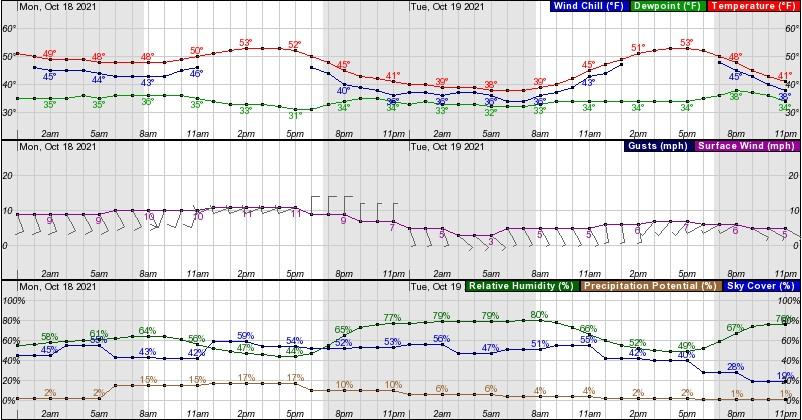
\includegraphics[width=0.8\linewidth]{https://sarakyeo.github.io/images/18-Oct-21_forecast} \end{center}
\end{frame}

\hypertarget{the-central-dogma-of-statistics}{%
\section{The Central Dogma of
Statistics}\label{the-central-dogma-of-statistics}}

\begin{frame}{}
\protect\hypertarget{section-6}{}
\begin{center}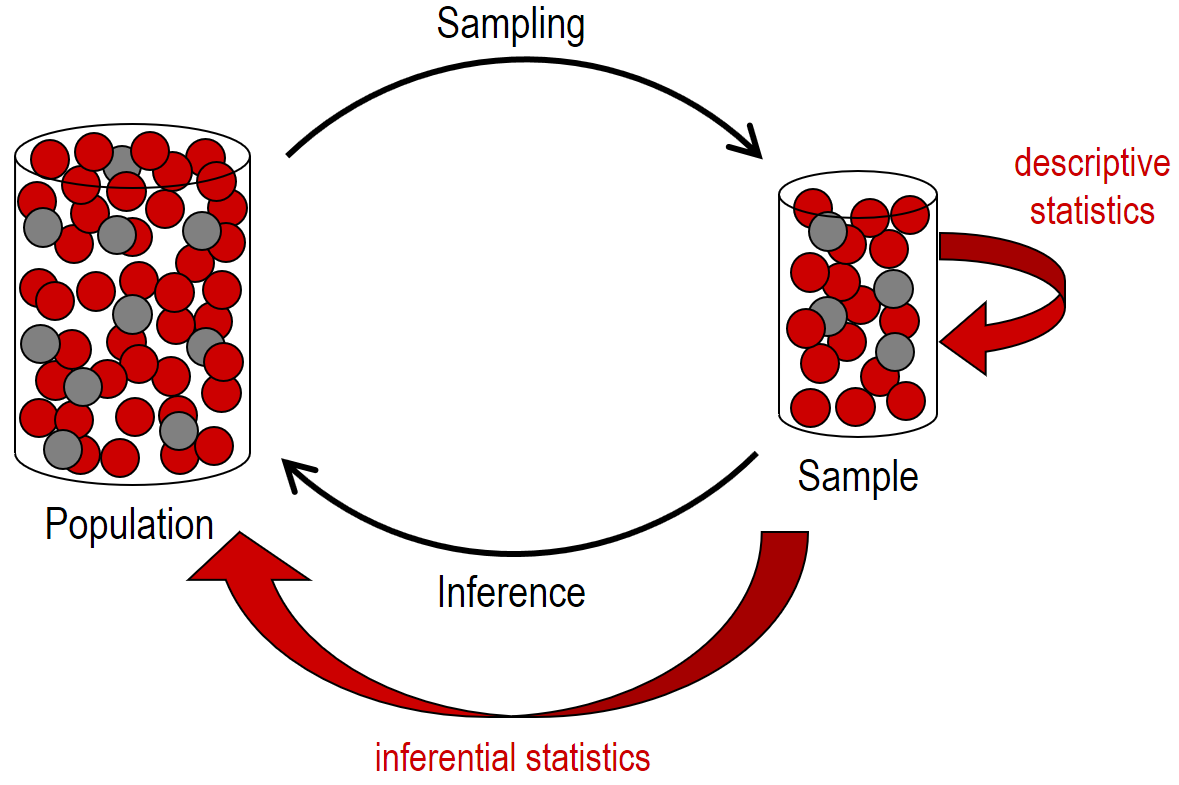
\includegraphics[width=0.8\linewidth]{https://sarakyeo.github.io/images/central-dogma-stats} \end{center}
\end{frame}

\begin{frame}{Using statistics, we want to learn about a
\emph{population}}
\protect\hypertarget{using-statistics-we-want-to-learn-about-a-population}{}
But, we rarely (if ever!) have access to every unit in a population.

Instead, we\ldots{}

\begin{itemize}[<+->]
\tightlist
\item
  take a representative sample, or a representative subset of the
  population, and
\item
  use this sample to \textbf{describe} (descriptive statistics) the
  population, and
\item
  we can also make \textbf{inferences/predictions/generalizations}
  (inferential statistics) about the population.
\end{itemize}
\end{frame}

\begin{frame}{}
\protect\hypertarget{section-7}{}
Recall that in our lecture on \textbf{Sampling}, we briefly defined the
term, \textbf{parameter}.

After reading this section, revisit
\href{https://sarakyeo.github.io/COMM-3710/week8.html}{the lecture from
Week 8} to see if the definitions of the terms, \emph{confidence
interval} and \emph{confidence level}, make more sense.
\end{frame}

\begin{frame}{But what exactly is a statistic? \textbar{} Let's look at
that figure again\ldots{}}
\protect\hypertarget{but-what-exactly-is-a-statistic-lets-look-at-that-figure-again}{}
\begin{center}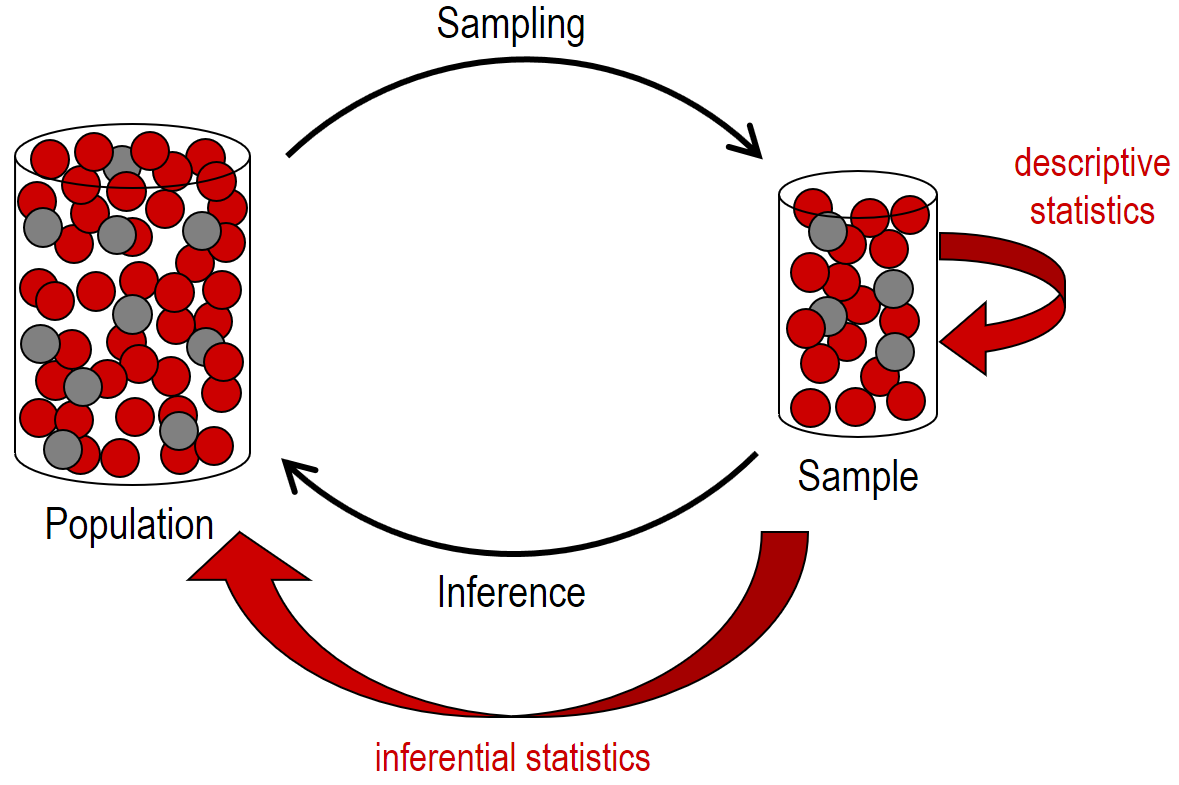
\includegraphics[width=1\linewidth]{https://sarakyeo.github.io/images/central-dogma-stats} \end{center}

Notice that the central dogma consists of a population and a sample.

\begin{itemize}[<+->]
\tightlist
\item
  \textbf{Statistics} are numbers that describe characteristics of
  \textbf{samples}.
\item
  \textbf{Parameters} describe \textbf{populations}.
\end{itemize}
\end{frame}

\begin{frame}{We use statistics from a sample to estimate (infer)
parameters in a population}
\protect\hypertarget{we-use-statistics-from-a-sample-to-estimate-infer-parameters-in-a-population}{}
Recall (from \href{https://sarakyeo.github.io/COMM-3710/week8.html}{Week
8}) that a \textbf{sample} consists of the units (in the case of survey
research, people) that are included in a study.

The \textbf{population}, on the other hand, is the entire group in which
a researcher is interested.

The population is a theoretically specified aggregation of the units
(i.e., people) in the study.
\end{frame}

\begin{frame}{The population is theoretical \textbar{} So instead we
collect a sample from the population}
\protect\hypertarget{the-population-is-theoretical-so-instead-we-collect-a-sample-from-the-population}{}
If you were interested in knowing the average height of adults in the
U.S., you would\ldots{}

\begin{itemize}
\tightlist
\item
  collect a sample that is representative of all American adults,
\item
  measure their individual heights, and
\item
  calculate a mean from this sample.
\end{itemize}

The calculated mean provides an estimate of the same parameter in the
population.
\end{frame}

\hypertarget{summary-population-parameter-vs.-sample-statistic}{%
\section{Summary: Population Parameter vs.~Sample
Statistic}\label{summary-population-parameter-vs.-sample-statistic}}

\begin{frame}{Parameter}
\protect\hypertarget{parameter}{}
\begin{itemize}[<+->]
\tightlist
\item
  number that describes the \textbf{population} (e.g., mean, standard
  deviation, variance, etc.)
\item
  parameters are often unknown because we cannot directly examine the
  entire population of interest!
\end{itemize}
\end{frame}

\begin{frame}{Statistic}
\protect\hypertarget{statistic}{}
\begin{itemize}[<+->]
\tightlist
\item
  number that can be computed from \textbf{sample} data (e.g., mean,
  standard deviation, variance, etc.)
\item
  we use statistics in a sample to estimate parameters in a population!
\item
  for example, we can calculate the mean age in a sample and use this
  statistic to estimate the mean age in the population.
\end{itemize}
\end{frame}

\hypertarget{descriptive-vs.-inferential-statistics-a-brief-introduction}{%
\section{Descriptive vs.~Inferential Statistics: A Brief
Introduction}\label{descriptive-vs.-inferential-statistics-a-brief-introduction}}

\begin{frame}{}
\protect\hypertarget{section-8}{}
In general, there are two types of statistics: \textbf{descriptive} and
\textbf{inferential} statistics.

\begin{center}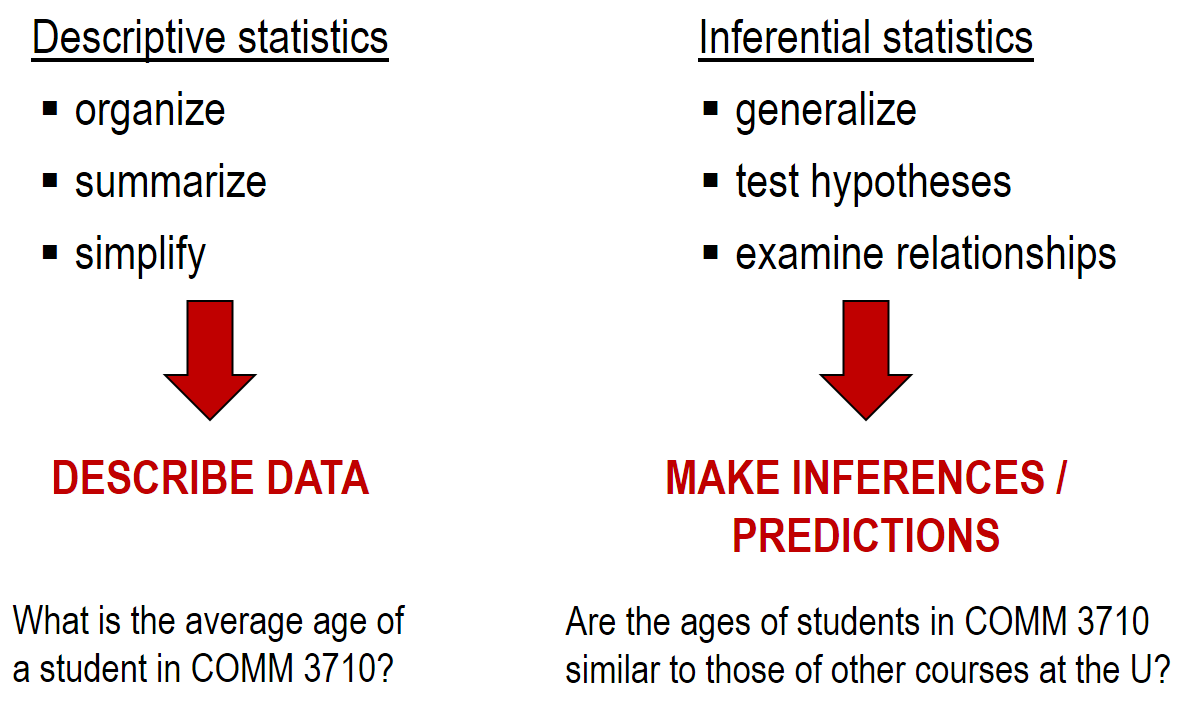
\includegraphics[width=0.8\linewidth]{https://sarakyeo.github.io/images/desc-infer-stats} \end{center}
\end{frame}

\begin{frame}{Descriptive statistics provide researchers with a
\emph{description} of what ``exists'' in the data}
\protect\hypertarget{descriptive-statistics-provide-researchers-with-a-description-of-what-exists-in-the-data}{}
Use the table below to calculate the \% of Americans who live in UT and
CA.

\begin{table}

\caption{\label{tab:unnamed-chunk-2}Population estimates for states in the western United States. Data from 2020 U.S. Census.}
\centering
\fontsize{20}{22}\selectfont
\begin{tabular}[t]{l|r}
\hline
USA & 334,735,155\\
\hline
Arizona & 7,151,502\\
\hline
California & 39,538,223\\
\hline
Colorado & 5,773,714\\
\hline
Idaho & 1,839,106\\
\hline
Montana & 1,084,225\\
\hline
Nevada & 3,104,614\\
\hline
New Mexico & 2,117,522\\
\hline
Oregon & 4,237,256\\
\hline
Utah & 3,271,616\\
\hline
Wyoming & 576,851\\
\hline
\end{tabular}
\end{table}
\end{frame}

\begin{frame}{}
\protect\hypertarget{section-9}{}
Approximately 1\% of the American population lives in Utah while 12\%
live in California.

\begin{itemize}
\tightlist
\item
  This comparison would be difficult without descriptive statistics.
\end{itemize}

We will focus on descriptive statistics next week.
\end{frame}

\begin{frame}{Inferential statistics is often a more advanced stage in
data analysis}
\protect\hypertarget{inferential-statistics-is-often-a-more-advanced-stage-in-data-analysis}{}
We use inferential statistics when we want to make \textbf{predictions}.

To make predictions, researchers often use inferential statistics to
draw conclusions and make predictions about a larger group (i.e., the
\textbf{population}) based on a smaller group of data (i.e., the
\textbf{sample}).

We will discuss inferential statistics more in a couple of weeks.
\end{frame}

\end{document}
